
\chapter{Architecture / Implementation}
\label{ch:implementation}

The Graphinius Platform consists of four main components as depicted in the following diagram. Of those 4, the practical parts of this Master thesis mainly consider Graphinius Base, with all graph construction and analysis functionality residing in GraphiniusJS. 

% \vspace{-0.5cm}
\begin{figure}[H]
	\centering
	\hspace*{-0.5cm}
	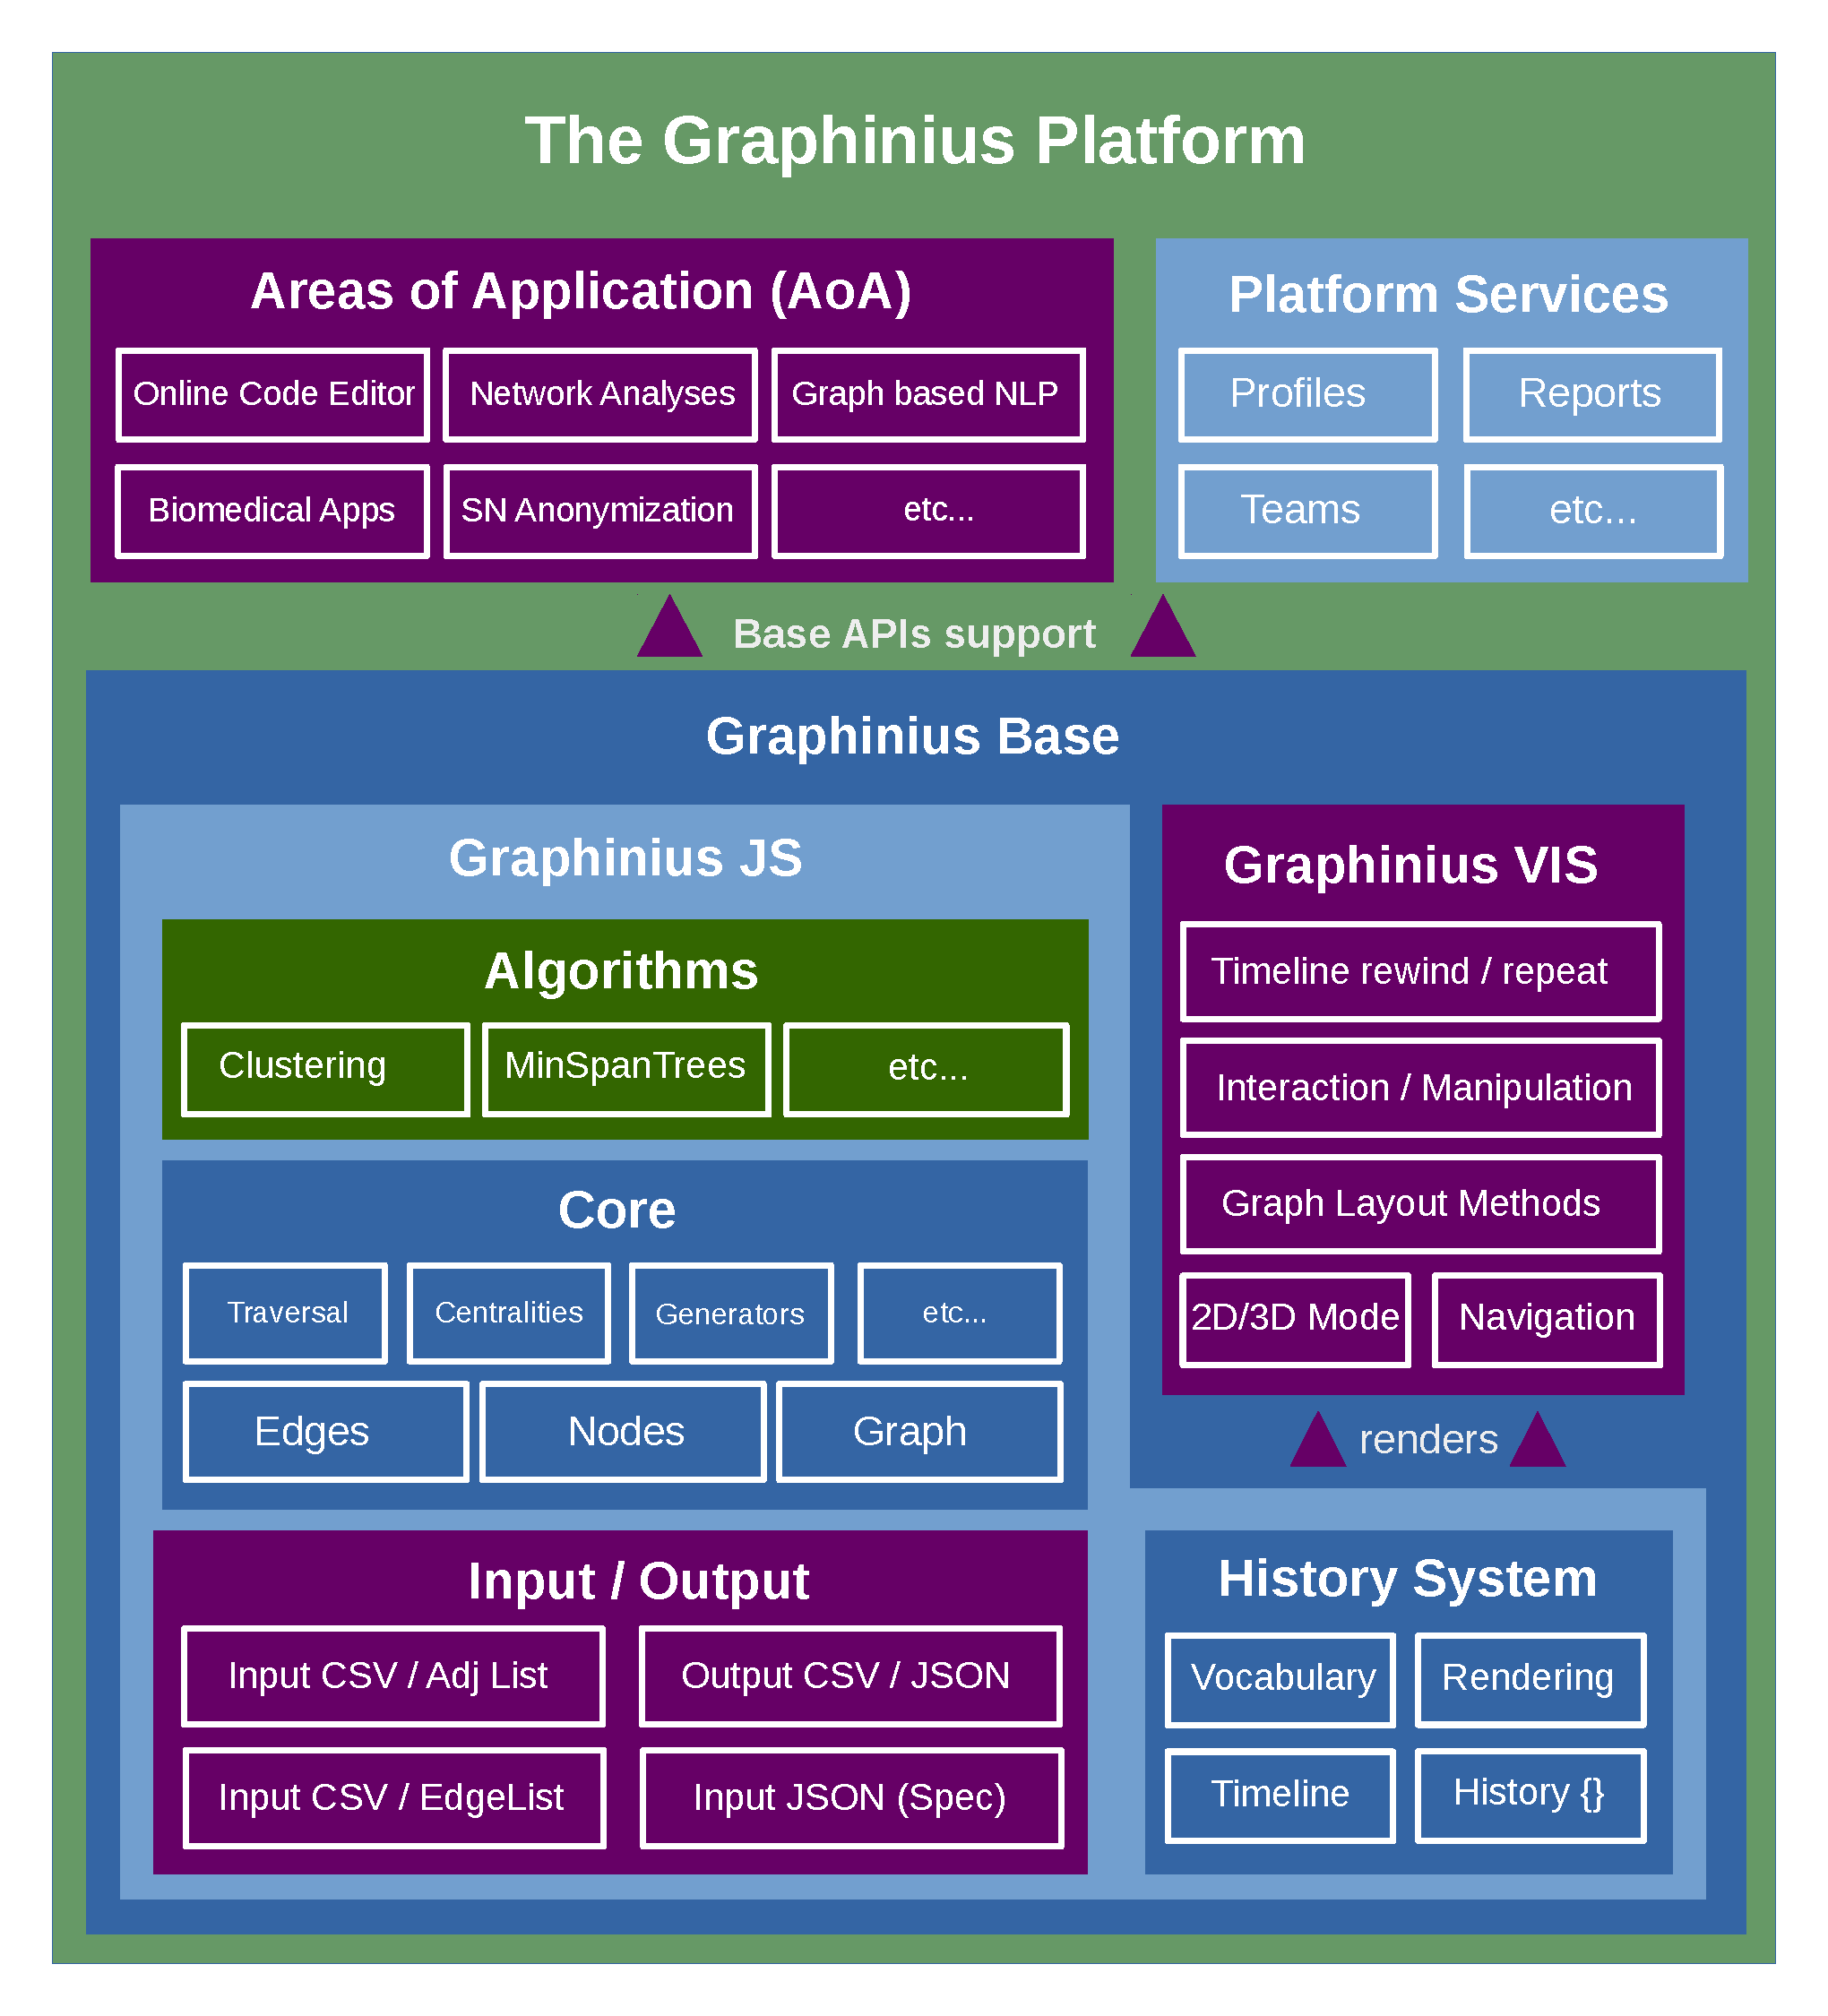
\includegraphics[width=1.05\textwidth]{figures/Graphinius_Architecture_new}
	\caption{Graphinius platform architecture overview}
	\label{fig_graphinius_architecture}
\end{figure}


\section{Graphinius Base}
\label{sect:graphinius_base}

As the name suggests, the Base module offers all the functionality necessary to develop graph-based applications on top of it, including basic graph-computations and algorithms as well as real-time, in-browser visualization. It is therefore logically composed of the two main modules \textit{GraphiniusJS} and \textit{GraphiniusVIS} as well as a mechanism of communication between those two, the \textit{History System}.


\section{Graphinius JS}
\label{sect:graphinius_js}

	\subsection{Graph Core}
	\label{ssect:graph_core}
		
		\subsubsection{Edges}
		\label{sssection: core_edges}
		
		\subsubsection{Nodes}
		\label{sssection: core_nodes}
		
		\subsubsection{Graph}
		\label{sssection: core_graph}
		
		\subsubsection{Generators}
		\label{sssection: core_}
		
		probability
		per-node degree
		
		\subsubsection{Degrees}
		\label{sssection: core_degrees}
		
		\subsubsection{Traversal - Breadth first search}
		\label{sssect:search_bfs}
		
		\subsubsection{Traversal - Depth first search}
		\label{sssect:search_dfs}
		
		\subsubsection{Traversal - Best (priority) first search}
		\label{sssect:search_pfs}
		
		\subsubsection{Traversal-based algorithms}
		\label{sssect:travseral_algos}
		
		Centralities are 
		
		BFS / DFS implementations... [figure: callback-based DFS]

	
	\subsection{Input / Output}
	\label{ssect:input_output}
	
	There are two basic input readers implemented in GraphiniusJS: 
	
	\textbf{The CSV Reader}, which takes adjacency lists or edge lists in CSV format and supports the most simple, but widely used, formats as well a a few additional options, and
	\textbf{The JSON Reader}, which operates on a custom, Graphinius-related JSON file format in order to support additional features specific to the use cases of the platform.
	
	As of the time of this writing, standard output filters have not been implemented, but would follow the same principles outlined below for their input counterparts.
		
		
		\subsubsection{CSV Reader}
		\label{sssection: io_csv}
		
		The CSV Reader class supports to widely used graph representation formats, namely \textit{adjacency lists} and \textit{edge lists}. An adjacency list is usually composed of lines indicating a StartNode at position one, followed by a series of connected EndNodes at the following positions in the line, where the connections can be interpreted as either directed or undirected edges:
		
		\begin{lstlisting}[caption={Sample Adjacency list, no edge direction.}, label={lst:adj_list_nodir}, language=JavaScript]
		A, B, C, A, D
		B, A
		C, A
		D, A
		\end{lstlisting}
		
		In addition to that, the Graphinius CSV Reader can be configured to consider explicitly defined edge directions, as in the following listing, or instructed to interpret all edges as either directed or undirected regardless of the direction specified in a file.
		
		\begin{lstlisting}[caption={Sample Adjacency list including edge direction.}, label={lst:adj_list_dir}, language=JavaScript]
		A, B, u, C, u, A, d, B, d, D, d
		B, A, u
		C, A, u, A, d
		D, A, d
		\end{lstlisting}
		
		CSV Edge Lists work analogously but are even simpler and use the format \textit{(StartNode, EndNode [,directed])}.	
		
		
		\subsubsection{JSON reader}
		\label{sssection: io_json}
		
		The Graphinius JSON reader is a more complex class as it uses it's own data format specific to the use cases targeted by the platform. It uses a nested object structure defining an array of node objects potentially containing different arrays of sub-objects:
		
		An \textbf{edge array} containing objects specifying a \textit{to} node, a \textit{direction} specifier as well as some \textit{weight}; direction and weight are optional; a \textbf{coordinates} array containing the \textit{x}, \textit{y}, and \textit{z} coordinates of a node; the \textit{z} coordinate is optional; a \textbf{feature vector} containing a hashmap of arbitrary length containing objects of arbitrary type including nested structures. The feature vector is solely used by applications building on GraphiniusJS and ignored by the standard suite of algorithms as described in the previous section.
		
		\begin{figure}[ht]
			\centering
			\hspace*{-1.5cm}
			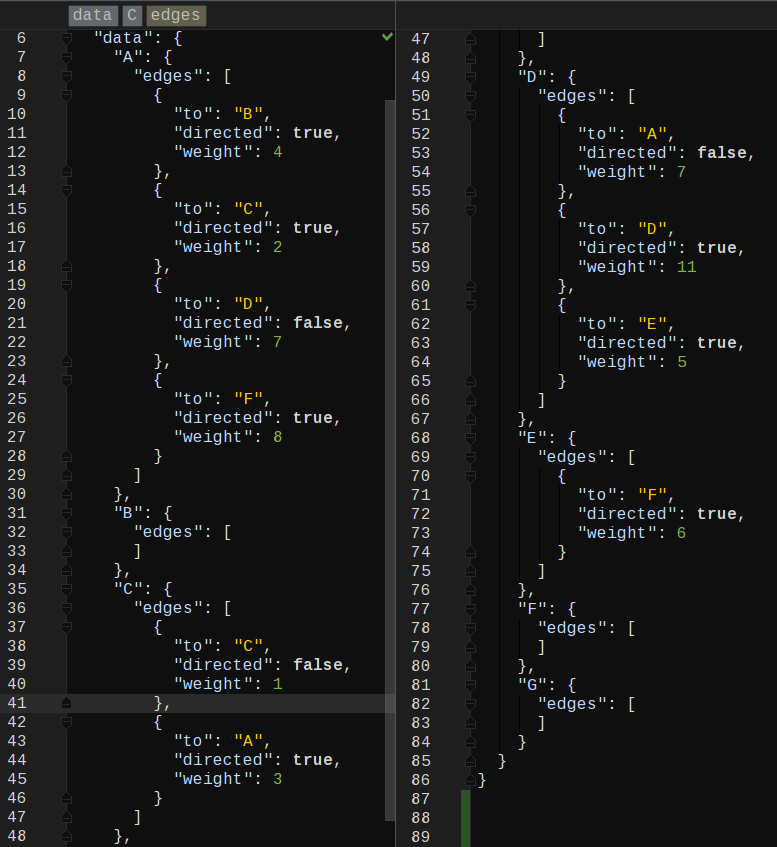
\includegraphics[width=1.2\textwidth]{figures/search_graph_json}
			\caption{Sample graph in the Graphinius JSON format}
			\label{fig:json_input_graph}
			\small Apart from the 'to' node, direction and weight, any node can exhibit an arbitrarily large feature vector containing any type of information (like patient data, word vectors, etc.). Another special sub-object which the input reader is looking for is the 'coords' object, which specifies the coordinates used in the constant layout renderer of the GraphiniusVIS library.
		\end{figure}



\section{The History system}
\label{sect:op_log}

	The idea of a history subsystem came from the concept of a real-time in-browser graph exploration platform, in which every action performed via an online editor or some GUI action should result in some immediate, visible change in the graph visualization. Ideally, such real-time changes would also be reversible, so that a user could progress step-by-step forward and backward in time - either to grasp more clearly what some algorithm does to the structure of a graph, or to 'simulate' the behavior of an algorithm on the whole. 
	
	In order to guarantee smooth behavior as well as separation of concerns in the software, placing this functionality directly in either the GraphiniusJS or GraphiniusVIS libraries would violate sound architectural principles. Therefor, the author proposes (but has not implemented yet) the following general module:
	
	\begin{landscape}
		\begin{figure}[ht]
			\label{fig_history_workflow}
			\centering
			\vspace{-2.0cm}
			%	\hspace*{0cm}
			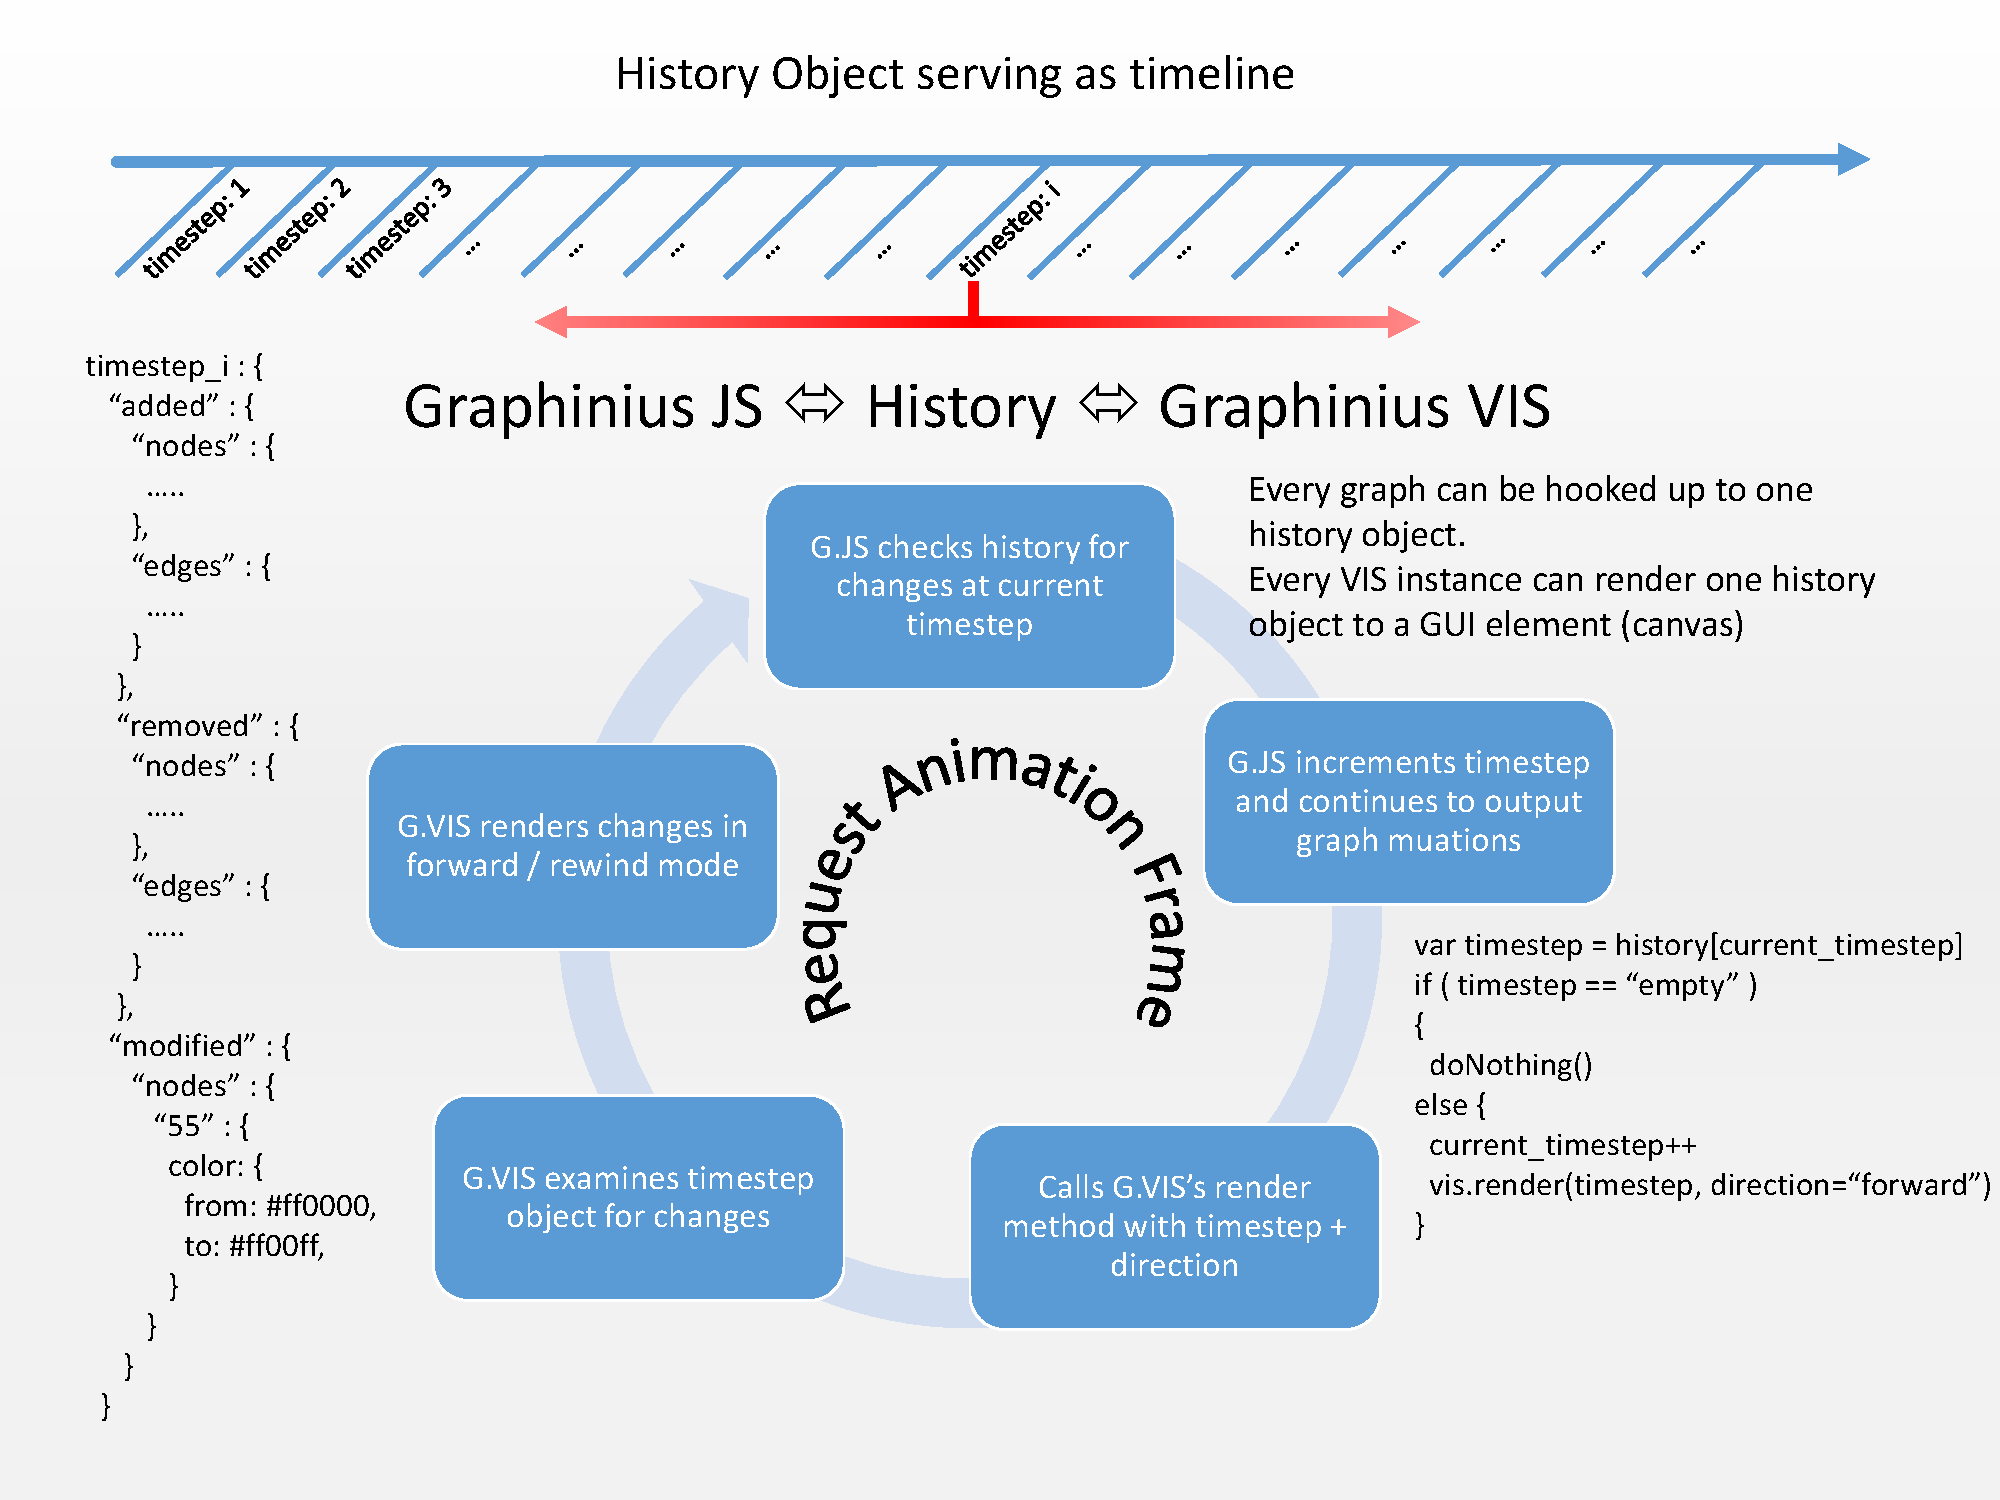
\includegraphics[width=1.6\textwidth]{figures/History_Workflow_pdf}
			\caption{Graphinius JS <-> VIS communication via Op-Log}
		\end{figure}
	\end{landscape}

	\subsection{Timeline}
	\label{ssect:timeline}
	
	The basic idea in implementing the system is to organize all graph mutations along the time axis, if only to imply chronological order. While it is less important to be able to specifically 'audit' some action in the sense of being able to exactly locate its temporal occurrence, we need some mapping of actions to a timestep (object) in order to be able to traverse the timeline back and forth. This is what determines the structure of the history object.
	
	\subsection{History Object}
	\label{ssect:history_object}

	The history object is a simple JavaScript object (which behaves like a hashmap in other languages' vocabulary) and holds entries in the form of \textit{timestep(timestep:number => actions:JSObject)}. These actions sub-objects then contain all the mutations which took place at a certain \textit{timestep}. It is important to realize that this \textit{timestep} is not an exact moment in time, but can span an arbitrarily long interval. Its value is determined by a global \textit{timestep} variable, which is only incremented when the rendering of the currently 'active' timestep has commenced. The actual procedure take the form of the following loop:
	
	\begin{enumerate}
		\item Graphinius Platforms runs recursive calls to \textit{window.requestAnimationFrame(renderFunc)} which simulates a main GUI loop
		\item At the beginning of each invocation, the algorithm checks for the current value of the global \textit{timestep} variable, and checks if the respective entry in the history object is empty or populated.
		\item In case it is empty, the algorithm breaks, laying inactive until the next time-tick from requestAnimationFrame (16.67 milliseconds on a 60Hz monitor).
		\item In case it is populated, the algorithm increments the global \textit{timestep} value - from this point onwards, GraphiniusJS will not write to that entry any more ('locking' it so that the rendering process can finish).
		\item All items in the current \textit{timestep} object will be evaluated resulting in calls to the GraphiniusVIS library updating the in-browser visualization.
	\end{enumerate}
	
	In order to be able to replay / rewind the mechanism, the history subsystem must have a sense of direction in time - which in our case simply translates to possessing a vocabulary expressing graph mutations in such a way that the respective inverse function is easily obtainable.
	
	\subsection{Vocabulary}
	\label{ssect:vocabulary}
	
	In order to achieve this, the \textit{timestep} entries must be as simple and specific as possible. For most of the primitive graph mutations, this is practically going to happen automatically: For instance, given the command \textit{'addNode(nodeId, arguments)'}, the inverse is logically \textit{'deleteNode(nodeId)'}. For more complex actions like changing coordinates, colors or shape, the original values would have to be stored. In the case of actions regarding whole clusters or changing the structure of the entire graph (\textit{run mincut..}), the \textit{timestep} entries will have to be broken down into atomic units and inverse actions defined in beforehand.


\section{Graphinius VIS}
\label{sect:graphinius_vis}

	The author was fortunate to receive the opportunity to guide the Master's Project of Nicole Neuhold in implementing a visualization module for the emerging Graphinius platform. We were working on research, experiments, and the foundation of a future implementation from early January 2016 to the end of March of the same year, and I am proud to be able to say that we surpassed our initial expectations - in brevity and conciseness of implementation as well as performance - by leaps and bounds and are not able to visualize graphs of 15k nodes / 40k edges fluently (~25 FPS) even on middle class laptops (22k nodes / 65k edges fluently on the author's desktop machine featuring a low-middle-class Geforce 650TI with 2GB of video RAM).
	
	\subsection{WebGL rendering}
	\label{ssect:webgl_rendering}
	
	The core component of the GraphiniusVIS module is the WebGL renderer. Although we experimented with SVG and Canvas (2D) as well, we quickly realized that both alternatives were either too slow or didn't provide us with the experience we desired: SVG has the great advantage of working with normal browser (DOM) objects, which enables easy interaction and selection via JS / CSS selectors, but stops rendering fluently at only a few hundred nodes / a few thousand edges.
	
	Canvas, on the other hand, is fine and fast enough for visualizing logical graph structures of thousands of nodes / edges in 2D. Nevertheless, because our project originated from the need to render structures  inherently 3D (like nevi and organs) and there was no easy possibility to project a 3D space onto a 2D canvas (except for computing the projection ourselves), we finally decided against it.
	
	Our Three.js / WebGL based renderer now uses low-level data structures like buffer geometries, statically typed JavaScript arrays and particle systems instead of 3D objects for nodes, which enables us to transfer our (pre-)computed data to the GPU in one single copy operation - this alone increases performance easily 10-fold over earlier attempts at progressively adding new objects to the scene.
	
	\subsection{2D/3D Mode}
	\label{ssect:vis_2d3d}
	
	GraphiniusVIS supports both 2D and 3D visualization of graph structures. However, since we are using WebGL which is inherently 3D, when switching to 2D mode we are not falling back to SVG or canvas but instead just 'fix' all z-coordinates of nodes / edges to zero, so we end up with a 2D object floating in 3D space.
	
	\subsection{Navigation}
	\label{ssect:vis_navigation}
	
	Our module supports panning (via mouse click-and-move), zooming (via mouse-wheel), rotating (via Shift + mouse click-and-move), and also provides any of those actions via keyboard commands.
	
	\subsection{Graph Layouts}
	\label{ssect:vis_layouts}
	
	The field of graph drawing has been an active area of research for several decades now, and many graph layouts have been developed for diverse areas of applications. Apart from constant (coordinate-based) layouts and force-directed layouts for physical simulations, there exist circular, spherical, tree-based, and arc diagrams, to name only a tiny fraction. Our basic implementation supports a constant layout per default, and allows switching to a force-directed layout as well, although the latter is currently implemented as a simple mathematical sine function instead of making use of attracting / repulsive forces.
	
	\subsection{Interaction / Manipulation}
	\label{ssect:vis_interact_manipulate}
	
	There are almost endless possibilities to interact with and manipulate a graph structure, so we were limited to offering just a small selection in order to demonstrate the viability of our GraphiniusVIS module. We chose to implement node and edge addition as well as deletion, changing the color of nodes and edges, updating their coordinates as well as switching from constant to our (simplified) force-directed layout. 
	
	In addition to that, in order to demonstrate seemless interaction (without a history object for now) between GraphiniusJS and GraphiniusVIS, one can visualize distances computed by BFS as well as segments computed by DFS (on a directed graph) from any random or chosen node. This even works during constant re-rendering in force-directed mode, although the algorithm is not yet implemented as a background thread (WebWorker / WebAssembly) and therefore causes the animation to lag for a fraction of a second.
	
	The following diagram summarizes some demo interactions / control flows contained in our base implementation.
	
	%\begin{landscape}
		\begin{figure}[ht]
			% \centering
			\hspace*{-1.3cm}
			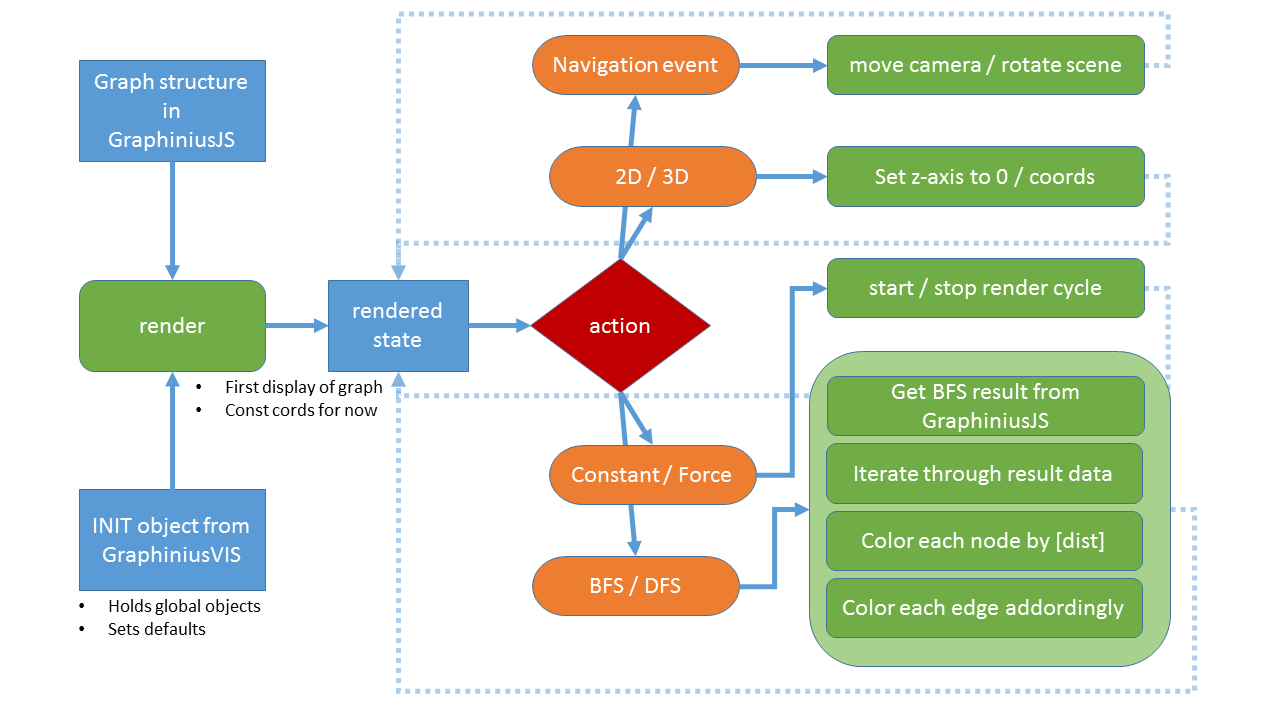
\includegraphics[width=1.2\textwidth]{figures/VIS_Control_Flow}
			\caption{Graphinius VIS control flow}
			\label{fig_vis_control_flow}
		\end{figure}
	%\end{landscape}


\section{Dependent Libraries}
\label{sect:dep_libraries}

	As described in the last chapter~\ref{ch:software_requirements}, modern web development processes utilize a wealth of external modules and helpers to achieve a seamless, convenient development workflow. Whereas GraphiniusJS does not depend on any external libraries at runtime (as can be seen in the \textit{"dependencies"} section of Figure~\ref{fig:dependencies}), the author has been using a diverse collection of dependencies at development time, which shall be only introduced in all brevity:
	
	The \textbf{chai} library handles assertions in mocha tests, \textbf{gulp} is the main taskrunner library, \textbf{gulp-clean} provides for deletion of compilation- and other results, \textbf{gulp-concat} manages file concatenations, \textbf{gulp-istanbul} integrates istanbul into the gulp process, \textbf{gulp-mocha} integrates mocha into the gulp process, \textbf{gulp-rename} handles renaming of one or many sources to a single destination file, \textbf{gulp-typedoc} integrates typedoc into the gulp process, \textbf{gulp-uglify} integrates uglify into the gulp process, \textbf{gulp-watch} provides file watching capabilities, \textbf{istanbul} provides test coverage reports, \textbf{jsdom} simulates a DOM environment in pure JavaScript (NodeJS), \textbf{jsdom-global} provides global variable support for jsdom, \textbf{json-loader} is a submodule of webpack allowing for integration of JSON files into a minified JS bundle, \textbf{merge2} merges file contents, \textbf{mocha} is the main test runner, \textbf{sinon} provides spies and stubs for testing, \textbf{sinon-chai} integrates sinon with the chai assertion library, \textbf{typedoc} automatically generates documentation from Typescript sources, \textbf{webpack-stream} is necessary for running a webpack process inside a (stream-based) gulp task, and \textbf{xhr-mock} provides a mocking service for simulating browser-based XMLHTTPRequest objects in server-side NodeJS.

	\begin{figure}[H]
		\centering
		\hspace*{-0.5cm}
		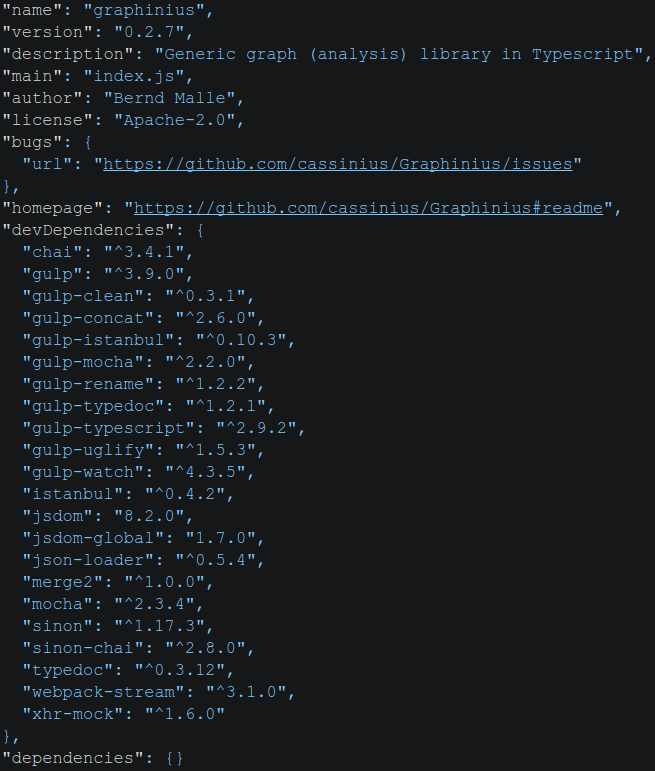
\includegraphics[width=1\textwidth]{figures/package_deps}
		\caption{GraphiniusJS development and runtime dependencies}
		\label{fig:dependencies}
	\end{figure}
	\small
	As is clearly visible, I focused on managing all complexity during development time, resulting in zero dependencies for the runtime JS bundle.


\section{Testing approach}
\label{sect:testing_approach}

	Behavior Driven Development (BDD) is a testing philosophy that approaches the development of a new feature from a high level view on the expected end-result and then works it's way down from spec's through functional to unit tests, until the feature is fully implemented, tested and covered. The ideal methodology would consist of the following steps:
	
	\begin{enumerate}
		\item Define the expected behavior of a feature (=module) in a form that both clients as well as developers understand and formulate them using (executable) specifications. The Cucumber framework introduced in the last chapter is an ideal candidate for this high level of abstraction. Executing the spec immediately will naturally fail because no code was actually written.
		\item From the specs defined in step one, we then derive functional tests which span the execution of several functions or methods in sequence in order to produce a certain result. Again, any test execution will expectedly fail as we have still not written the code yet.
		\item From the functional tests defined in step two, we finally derive low-level tests covering single units of code. Once more the tests will fail initially, upon which we endeavor to fill in the single pieces of code until all tests at that level are passing.
		\item Once the unit-test level is done, we work our way upwards to the next functional test on our todo-list. This process is repeated until all functional tests required for our initially specified features are covered.
		\item We then move on to the next feature on our product requirements list.
	\end{enumerate}
	
	 As already mentioned, because a software library intended to be used by other programmers usually has only technical clients, feature specification (testing) was omitted in programming Graphinius JS. For this reason, we will only take a look at unit and functional tests in this section (as well was mocking and spying). Furthermore, in developing a web application using the Mocha and Chai test libraries, there is no fundamental difference between unit and functional tests. Let us therefore take a look at instances of both categories to see how we would structure our approach:
	
	\subsection{Unit tests}
	\label{ssect:unittests}
	
	As stated, unit tests cover the low-level constructs of functions or methods which themselves do not depend on any lower-level functions.
	
	In the example below, we see two test cases: the first calls a binary Heap evalInputPriority function on line 2, whose job it is to cast any input to a (sortable) number, if possible. As the string "55" can be cast to the number 55, this test will be successful. In the second example on lines 5 and 6, we pass boolean values which - employing the JS \textit{parseInt(arg)} function - will evaluate to NaN (which is JS shorthand for \textit{Not a Number}).
	
	\begin{lstlisting}[caption={Unit tests covering the functionality of one simple function.}, label={fig:unit_tests}, language=JavaScript]	
it('should accept String encoded Integers as input and evaluate to their Integer value', () => {
	expect(binHeap.evalInputPriority("55")).to.equal(55);
});
it('should not accept booleans as input values (makes no sense...) ', () => {
	expect(binHeap.evalInputPriority(true)).to.be.NaN;
	expect(binHeap.evalInputPriority(false)).to.be.NaN;
});
	\end{lstlisting}
	\small
	(Sample taken from the GraphiniusJS binaryHeapTests.ts file.)
	
	
	\subsection{Functional tests}
	\label{ssect:func_tests}
	
	In functional testing we invoke some procedure which in turn will call other functions or methods, in any sequence or call depth required in order to fulfill its purpose.
	
	In the example below, we instantiate a new JSON reader, specify some configuration options and hand it a JSON file. We then expect the resulting graph to be of a certain size in number of nodes and edges. The \textit{readFromJSONFile} function will itself call several subordinate functions for reading a file from disk, processing the character sequence it receives, instantiating a GraphiniusJS graph object etc.
	
	\begin{lstlisting}[caption={A functional test covering the whole instantiation process of a graph from a JSON input structure.}, label={fig:functional_test}, language=JavaScript]
it('should correctly generate our small example graph out of a JSON file with direction _mode set to undirected', () => {
	json = new JSON_IN();
	json._explicit_direction = false;
	json._direction = false;
	graph = json.readFromJSONFile(small_graph);
	expect(graph.nrNodes()).to.equal(4);
	expect(graph.nrDirEdges()).to.equal(0);
	expect(graph.nrUndEdges()).to.equal(4);
});
	\end{lstlisting}
	\small
	(Sample taken from the GraphiniusJS JSONInputTests.ts file.)
	
	
	\subsection{Mocks used for browser code testing}
	\label{ssect:mocks}
	
	Mocks are a useful construct for testing functionality that would involve some non-trivial behavior. For instance, if we would like to test a snippet of code (as in the following code example) which loads a JSON file remotely over the network before instantiating a graph, we are assuming the existence of a server, the existence of the remote file, as well as a working Internet connection. Moreover, in this specific case, the code under test is also meant to be executed inside a browser environment, whereas we would like to invoke our test from the NodeJS console.
	
	The solution to this problem is to \text{mock} the XMLHTTPRequest object used by a browser to send AJAX requests over the internet, which - again in this specific case - replaces the object with a NodeJS request object and simulates the original XMLHTTPRequest API through a delegating wrapper around it. The exact sequence in this example is: 1) requiring the mocking library on line 3, 2) initializing a browser environment (providing the window and document objects) on line 4, 3) injecting browser globals into the Node environment on line 13, 4) requiring filesystem capabilities for local file loading on line 16 as well as loading the file on line 17, 5) initiating the mock on line 20 and finally setting up a fake web server responding to a certain URL on lines 23 through 30. The rest of the procedure (not shown in this exmaple) behaves exactly as an equivalent test inside a browser environment would.
	
	\begin{lstlisting}[caption={A mocking setup simulating a Web Server GET response...}, label={fig:mock_service_test}, language=JavaScript]
describe('Loading graphs in simulated browser environment', () => {		
	// Mocking the XHR object
	var mock = require('xhr-mock');
	var jsDomCleanup = null,
	mocked = false;
	
	// URL to replace with path
	var small_graph_url = REMOTE_HOST + "small_graph.json";
	var small_graph_path = 'test/input/test_data/small_graph.json';
	
	beforeEach(() => {		
		// Injecting browser globals into our Node environment
		jsDomCleanup = require('jsdom-global')();
		
		// Access to local filesystem for mocking service
		var fs = require('fs');
		var json = fs.readFileSync(small_graph_path).toString();
		
		//replace the real XHR object with the mock XHR object
		mock.setup();
	
		// Mocking Browser GET request to test server
			mock.get(small_graph_url, function(req, res) {
				mocked = true;
				return res
					.status(200)
					.header('Content-Type', 'application/json')
					.body(json);
			});
		});
		
	afterEach(() => {
		mock.teardown();
		jsDomCleanup();
		mocked = false;
	});
	
	// Rest of tests are the same as in non-mocked, local reader based input tests
});
	\end{lstlisting}
	\small
	... to an XML-HTTP GET Request in order to read a graph structure from a remote JSON file from inside a browser environment. (Sample taken from the GraphiniusJS JSONInputAsyncTests.ts file.)
	
	
	\subsection{Stubs}
	\label{ssect:stubs}
	There is another concept often confused with mocks called \textit{stubs}. Stubs are used when the response of a function is not supposed to be complex but rather boolean in nature. E.g. an authorization module could internally use a method checking if a user has sufficient permissions to be allowed to access a resource. This functionality could be implemented rather simply, or it could invoke elaborate tests involving diverse software modules throughout the whole system. For testing some function building upon it however, only the distinction between \textit{allowed} and \textit{not allowed} is are really of interest. Therefore, a stub can be instantiated and told to forgo any \textit{real} authority checks but instead simply return a true or false value. 
	
	The difference between stubs and mocks is therefore that stubs replace potentially complex implementations with trivial ones, whereas mocks can act as a proxy but do not necessarily reduce complexity - reading a graph from a local file is as complex as reading it from a remote one (not considering the underlying complexity of the network stack, of course).
	

	\subsection{Spies (Sinon)}
	\label{ssect:spies}
	
	Spies are test wrapper objects that observe the original function or method and record any activity regarding it, e.g. how often it was called, which argument values it was called with, which values were returned or if an error was thrown. In the example below, we instantiate a local backup object \textit{original}, then instantiate a spy on line 10, store the original function reference in our backup object on line 12, and replace the original function with our spy on line 14. In calling \$DFS.prepareDFSVisitStandardConfig on line 25, we expect to see the original function invoked in the process, which we check on line 28. The \textit{after} block from lines 18 through 21 then restores the original objects.
	
	\begin{lstlisting}[caption={A functional test making use of a spy...}, label={fig:spy_test}, language=JavaScript]
describe('testing config preparation functions - ', () => {
	var prepForDFSVisitSpy,
	prepForDFSSpy,
	original = {
		prepareDFSStandardConfig: null,
		prepareDFSVisitStandardConfig: null
	};

	before(() => {
		prepForDFSSpy = sinon.spy($DFS.prepareDFSStandardConfig);
		prepForDFSVisitSpy = sinon.spy($DFS.prepareDFSVisitStandardConfig);
		original.prepareDFSStandardConfig = $DFS.prepareDFSStandardConfig;
		original.prepareDFSVisitStandardConfig = $DFS.prepareDFSVisitStandardConfig;
		$DFS.prepareDFSStandardConfig = prepForDFSSpy;
		$DFS.prepareDFSVisitStandardConfig = prepForDFSVisitSpy;
	});

	after(() => {
		$DFS.prepareDFSStandardConfig = original.prepareDFSStandardConfig;      
		$DFS.prepareDFSVisitStandardConfig = original.prepareDFSVisitStandardConfig;
	});


	it('preprareDFSVisitStandardConfig should correctly instantiate a DFSConfig object', () => {
		var config = $DFS.prepareDFSVisitStandardConfig();
		
		// Here the spy is finally used to check internal method invocation
		expect(prepForDFSVisitSpy).to.have.been.calledOnce;
	});
});
	\end{lstlisting}
	\small
	... to test internal method invocation, restoring the original method afterwards. (Sample taken from the GraphiniusJS DFSTests.ts file.)

	
\section{Areas of Application}
\label{sect:aoas}

The implementation of 3 demo applications will be described in the next Chapter, Implementation - Areas of Application)~\ref{ch:use_cases}.
	
\section{Platform Services}
\label{sect:platform_services}

As of the time of this writing, the Graphinius Platform has not taken shape yet, so there is no available implementation to discuss.

%\subsection{Personal Profile}
%\label{ssect:service_profile}

%\subsection{Teams}
%\label{ssect:service_teams}

%\subsection{Output / Reports}
%\label{ssect:service_output}